
%% bare_conf_compsoc.tex
%% V1.4b
%% 2015/08/26
%% by Michael Shell
%% See:
%% http://www.michaelshell.org/
%% for current contact information.
%%
%% This is a skeleton file demonstrating the use of IEEEtran.cls
%% (requires IEEEtran.cls version 1.8b or later) with an IEEE Computer
%% Society conference paper.
%%
%% Support sites:
%% http://www.michaelshell.org/tex/ieeetran/
%% http://www.ctan.org/pkg/ieeetran
%% and
%% http://www.ieee.org/

%%*************************************************************************
%% Legal Notice:
%% This code is offered as-is without any warranty either expressed or
%% implied; without even the implied warranty of MERCHANTABILITY or
%% FITNESS FOR A PARTICULAR PURPOSE! 
%% User assumes all risk.
%% In no event shall the IEEE or any contributor to this code be liable for
%% any damages or losses, including, but not limited to, incidental,
%% consequential, or any other damages, resulting from the use or misuse
%% of any information contained here.
%%
%% All comments are the opinions of their respective authors and are not
%% necessarily endorsed by the IEEE.
%%
%% This work is distributed under the LaTeX Project Public License (LPPL)
%% ( http://www.latex-project.org/ ) version 1.3, and may be freely used,
%% distributed and modified. A copy of the LPPL, version 1.3, is included
%% in the base LaTeX documentation of all distributions of LaTeX released
%% 2003/12/01 or later.
%% Retain all contribution notices and credits.
%% ** Modified files should be clearly indicated as such, including  **
%% ** renaming them and changing author support contact information. **
%%*************************************************************************


% *** Authors should verify (and, if needed, correct) their LaTeX system  ***
% *** with the testflow diagnostic prior to trusting their LaTeX platform ***
% *** with production work. The IEEE's font choices and paper sizes can   ***
% *** trigger bugs that do not appear when using other class files.       ***                          ***
% The testflow support page is at:
% http://www.michaelshell.org/tex/testflow/



\documentclass[,conference,compsoc]{IEEEtran}
% Some/most Computer Society conferences require the compsoc mode option,
% but others may want the standard conference format.
%
% If IEEEtran.cls has not been installed into the LaTeX system files,
% manually specify the path to it like:
% \documentclass[conference,compsoc]{../sty/IEEEtran}





% Some very useful LaTeX packages include:
% (uncomment the ones you want to load)


% *** MISC UTILITY PACKAGES ***
%
%\usepackage{ifpdf}
% Heiko Oberdiek's ifpdf.sty is very useful if you need conditional
% compilation based on whether the output is pdf or dvi.
% usage:
% \ifpdf
%   % pdf code
% \else
%   % dvi code
% \fi
% The latest version of ifpdf.sty can be obtained from:
% http://www.ctan.org/pkg/ifpdf
% Also, note that IEEEtran.cls V1.7 and later provides a builtin
% \ifCLASSINFOpdf conditional that works the same way.
% When switching from latex to pdflatex and vice-versa, the compiler may
% have to be run twice to clear warning/error messages.

% set space package to adjust line spacing
\usepackage{setspace}

% add line numbers to both sides of the doucment
\usepackage[switch]{lineno}
\usepackage{blindtext}


% *** CITATION PACKAGES ***
%
\ifCLASSOPTIONcompsoc
  % IEEE Computer Society needs nocompress option
  % requires cite.sty v4.0 or later (November 2003)
  \usepackage[nocompress]{cite}
\else
  % normal IEEE
  \usepackage{cite}
\fi
% cite.sty was written by Donald Arseneau
% V1.6 and later of IEEEtran pre-defines the format of the cite.sty package
% \cite{} output to follow that of the IEEE. Loading the cite package will
% result in citation numbers being automatically sorted and properly
% "compressed/ranged". e.g., [1], [9], [2], [7], [5], [6] without using
% cite.sty will become [1], [2], [5]--[7], [9] using cite.sty. cite.sty's
% \cite will automatically add leading space, if needed. Use cite.sty's
% noadjust option (cite.sty V3.8 and later) if you want to turn this off
% such as if a citation ever needs to be enclosed in parenthesis.
% cite.sty is already installed on most LaTeX systems. Be sure and use
% version 5.0 (2009-03-20) and later if using hyperref.sty.
% The latest version can be obtained at:
% http://www.ctan.org/pkg/cite
% The documentation is contained in the cite.sty file itself.
%
% Note that some packages require special options to format as the Computer
% Society requires. In particular, Computer Society  papers do not use
% compressed citation ranges as is done in typical IEEE papers
% (e.g., [1]-[4]). Instead, they list every citation separately in order
% (e.g., [1], [2], [3], [4]). To get the latter we need to load the cite
% package with the nocompress option which is supported by cite.sty v4.0
% and later.





% *** GRAPHICS RELATED PACKAGES ***
%
\ifCLASSINFOpdf
  \usepackage[pdftex]{graphicx}
  % declare the path(s) where your graphic files are
  \graphicspath{{./img/}}
  % and their extensions so you won't have to specify these with
  % every instance of \includegraphics
  \DeclareGraphicsExtensions{.pdf,.jpeg,.png}
\else
  % or other class option (dvipsone, dvipdf, if not using dvips). graphicx
  % will default to the driver specified in the system graphics.cfg if no
  % driver is specified.
  % \usepackage[dvips]{graphicx}
  % declare the path(s) where your graphic files are
  % \graphicspath{{../eps/}}
  % and their extensions so you won't have to specify these with
  % every instance of \includegraphics
  % \DeclareGraphicsExtensions{.eps}
\fi
% graphicx was written by David Carlisle and Sebastian Rahtz. It is
% required if you want graphics, photos, etc. graphicx.sty is already
% installed on most LaTeX systems. The latest version and documentation
% can be obtained at: 
% http://www.ctan.org/pkg/graphicx
% Another good source of documentation is "Using Imported Graphics in
% LaTeX2e" by Keith Reckdahl which can be found at:
% http://www.ctan.org/pkg/epslatex
%
% latex, and pdflatex in dvi mode, support graphics in encapsulated
% postscript (.eps) format. pdflatex in pdf mode supports graphics
% in .pdf, .jpeg, .png and .mps (metapost) formats. Users should ensure
% that all non-photo figures use a vector format (.eps, .pdf, .mps) and
% not a bitmapped formats (.jpeg, .png). The IEEE frowns on bitmapped formats
% which can result in "jaggedy"/blurry rendering of lines and letters as
% well as large increases in file sizes.
%
% You can find documentation about the pdfTeX application at:
% http://www.tug.org/applications/pdftex





% *** MATH PACKAGES ***
%
\usepackage{amsmath}
\usepackage{amsfonts}
\usepackage{amssymb}
% A popular package from the American Mathematical Society that provides
% many useful and powerful commands for dealing with mathematics.
%
% Note that the amsmath package sets \interdisplaylinepenalty to 10000
% thus preventing page breaks from occurring within multiline equations. Use:
%\interdisplaylinepenalty=2500
% after loading amsmath to restore such page breaks as IEEEtran.cls normally
% does. amsmath.sty is already installed on most LaTeX systems. The latest
% version and documentation can be obtained at:
% http://www.ctan.org/pkg/amsmath





% *** SPECIALIZED LIST PACKAGES ***
%
\usepackage{algorithmic}
% algorithmic.sty was written by Peter Williams and Rogerio Brito.
% This package provides an algorithmic environment fo describing algorithms.
% You can use the algorithmic environment in-text or within a figure
% environment to provide for a floating algorithm. Do NOT use the algorithm
% floating environment provided by algorithm.sty (by the same authors) or
% algorithm2e.sty (by Christophe Fiorio) as the IEEE does not use dedicated
% algorithm float types and packages that provide these will not provide
% correct IEEE style captions. The latest version and documentation of
% algorithmic.sty can be obtained at:
% http://www.ctan.org/pkg/algorithms
% Also of interest may be the (relatively newer and more customizable)
% algorithmicx.sty package by Szasz Janos:
% http://www.ctan.org/pkg/algorithmicx




% *** ALIGNMENT PACKAGES ***
%
%\usepackage{array}
% Frank Mittelbach's and David Carlisle's array.sty patches and improves
% the standard LaTeX2e array and tabular environments to provide better
% appearance and additional user controls. As the default LaTeX2e table
% generation code is lacking to the point of almost being broken with
% respect to the quality of the end results, all users are strongly
% advised to use an enhanced (at the very least that provided by array.sty)
% set of table tools. array.sty is already installed on most systems. The
% latest version and documentation can be obtained at:
% http://www.ctan.org/pkg/array


% IEEEtran contains the IEEEeqnarray family of commands that can be used to
% generate multiline equations as well as matrices, tables, etc., of high
% quality.




% *** SUBFIGURE PACKAGES ***
%\ifCLASSOPTIONcompsoc
%  \usepackage[caption=false,font=footnotesize,labelfont=sf,textfont=sf]{subfig}
%\else
%  \usepackage[caption=false,font=footnotesize]{subfig}
%\fi
% subfig.sty, written by Steven Douglas Cochran, is the modern replacement
% for subfigure.sty, the latter of which is no longer maintained and is
% incompatible with some LaTeX packages including fixltx2e. However,
% subfig.sty requires and automatically loads Axel Sommerfeldt's caption.sty
% which will override IEEEtran.cls' handling of captions and this will result
% in non-IEEE style figure/table captions. To prevent this problem, be sure
% and invoke subfig.sty's "caption=false" package option (available since
% subfig.sty version 1.3, 2005/06/28) as this is will preserve IEEEtran.cls
% handling of captions.
% Note that the Computer Society format requires a sans serif font rather
% than the serif font used in traditional IEEE formatting and thus the need
% to invoke different subfig.sty package options depending on whether
% compsoc mode has been enabled.
%
% The latest version and documentation of subfig.sty can be obtained at:
% http://www.ctan.org/pkg/subfig




% *** FLOAT PACKAGES ***
%
\usepackage{multirow}
%\usepackage{fixltx2e}
% fixltx2e, the successor to the earlier fix2col.sty, was written by
% Frank Mittelbach and David Carlisle. This package corrects a few problems
% in the LaTeX2e kernel, the most notable of which is that in current
% LaTeX2e releases, the ordering of single and double column floats is not
% guaranteed to be preserved. Thus, an unpatched LaTeX2e can allow a
% single column figure to be placed prior to an earlier double column
% figure.
% Be aware that LaTeX2e kernels dated 2015 and later have fixltx2e.sty's
% corrections already built into the system in which case a warning will
% be issued if an attempt is made to load fixltx2e.sty as it is no longer
% needed.
% The latest version and documentation can be found at:
% http://www.ctan.org/pkg/fixltx2e


%\usepackage{stfloats}
% stfloats.sty was written by Sigitas Tolusis. This package gives LaTeX2e
% the ability to do double column floats at the bottom of the page as well
% as the top. (e.g., "\begin{figure*}[!b]" is not normally possible in
% LaTeX2e). It also provides a command:
%\fnbelowfloat
% to enable the placement of footnotes below bottom floats (the standard
% LaTeX2e kernel puts them above bottom floats). This is an invasive package
% which rewrites many portions of the LaTeX2e float routines. It may not work
% with other packages that modify the LaTeX2e float routines. The latest
% version and documentation can be obtained at:
% http://www.ctan.org/pkg/stfloats
% Do not use the stfloats baselinefloat ability as the IEEE does not allow
% \baselineskip to stretch. Authors submitting work to the IEEE should note
% that the IEEE rarely uses double column equations and that authors should try
% to avoid such use. Do not be tempted to use the cuted.sty or midfloat.sty
% packages (also by Sigitas Tolusis) as the IEEE does not format its papers in
% such ways.
% Do not attempt to use stfloats with fixltx2e as they are incompatible.
% Instead, use Morten Hogholm'a dblfloatfix which combines the features
% of both fixltx2e and stfloats:
%
% \usepackage{dblfloatfix}
% The latest version can be found at:
% http://www.ctan.org/pkg/dblfloatfix




% *** PDF, URL AND HYPERLINK PACKAGES ***
%
%\usepackage{url}
% url.sty was written by Donald Arseneau. It provides better support for
% handling and breaking URLs. url.sty is already installed on most LaTeX
% systems. The latest version and documentation can be obtained at:
% http://www.ctan.org/pkg/url
% Basically, \url{my_url_here}.




% *** Do not adjust lengths that control margins, column widths, etc. ***
% *** Do not use packages that alter fonts (such as pslatex).         ***
% There should be no need to do such things with IEEEtran.cls V1.6 and later.
% (Unless specifically asked to do so by the journal or conference you plan
% to submit to, of course. )


% correct bad hyphenation here
\hyphenation{op-tical net-works semi-conduc-tor}

% Adds page borders and file info (page number, date, filename, etc)
%\usepackage[a4,frame,center]{crop}

\begin{document}

% add line numbers
%\linenumbers

%
% paper title
% Titles are generally capitalized except for words such as a, an, and, as,
% at, but, by, for, in, nor, of, on, or, the, to and up, which are usually
% not capitalized unless they are the first or last word of the title.
% Linebreaks \\ can be used within to get better formatting as desired.
% Do not put math or special symbols in the title.
\title{Stochastic Repeated Gradient Descent (SRGD)}


% author names and affiliations
% use a multiple column layout for up to three different
% affiliations
\author{\IEEEauthorblockN{Jeff Hajewski}
\IEEEauthorblockA{
University of Iowa\\
Iowa City, Iowa\\
Email: jeffrey-hajewski@uiowa.edu}}

% conference papers do not typically use \thanks and this command
% is locked out in conference mode. If really needed, such as for
% the acknowledgment of grants, issue a \IEEEoverridecommandlockouts
% after \documentclass

% for over three affiliations, or if they all won't fit within the width
% of the page (and note that there is less available width in this regard for
% compsoc conferences compared to traditional conferences), use this
% alternative format:
% 
%\author{\IEEEauthorblockN{Michael Shell\IEEEauthorrefmark{1},
%Homer Simpson\IEEEauthorrefmark{2},
%James Kirk\IEEEauthorrefmark{3}, 
%Montgomery Scott\IEEEauthorrefmark{3} and
%Eldon Tyrell\IEEEauthorrefmark{4}}
%\IEEEauthorblockA{\IEEEauthorrefmark{1}School of Electrical and Computer Engineering\\
%Georgia Institute of Technology,
%Atlanta, Georgia 30332--0250\\ Email: see http://www.michaelshell.org/contact.html}
%\IEEEauthorblockA{\IEEEauthorrefmark{2}Twentieth Century Fox, Springfield, USA\\
%Email: homer@thesimpsons.com}
%\IEEEauthorblockA{\IEEEauthorrefmark{3}Starfleet Academy, San Francisco, California 96678-2391\\
%Telephone: (800) 555--1212, Fax: (888) 555--1212}
%\IEEEauthorblockA{\IEEEauthorrefmark{4}Tyrell Inc., 123 Replicant Street, Los Angeles, California 90210--4321}}




% use for special paper notices
%\IEEEspecialpapernotice{(Invited Paper)}




% make the title area
\maketitle

% As a general rule, do not put math, special symbols or citations
% in the abstract
\begin{abstract}
    Stochastic Repeated Gradient Descent (SRGD) is a derivative of mini-batched
    SGD that performs multiple parameter updates for a given mini-batch within a
    single training epoch. The goal of this approach is to capitalize on CPU
    cache to reduce the wait time between training iterations.
\end{abstract}

% no keywords




% For peer review papers, you can put extra information on the cover
% page as needed:
% \ifCLASSOPTIONpeerreview
% \begin{center} \bfseries EDICS Category: 3-BBND \end{center}
% \fi
%
% For peerreview papers, this IEEEtran command inserts a page break and
% creates the second title. It will be ignored for other modes.



\section{Introduction}
% no \IEEEPARstart
We introduce Stochastic Repeated Gradient Descent(SRGD), a modification to
Stochastic Gradient Descent that takes advantage of CPU cache to improve compute
time and allow the use of large mini-batches, resulting in dramatically faster
time to convergence versus mini-batch SGD. 

Stochastic Gradient Descent (SGD) has long been the standard optimization method
in machine learning. Recent developments such as Adam and AdaGrad solve some of
the shortcomings of SGD by using adaptive learning rates and scaled gradients.
While these methods have seen substantial success, they can suffer from
increased storage requirements, which is problematic for large problems.
Additionally, they can be more challenging to implement, as the algorithms are
more complex than standard SGD. Stochastic Repeated Gradient Descent aims to
reduce compute time by taking advantage of CPU cache and allowing the use of
larger mini-batch sizes without degrading convergence results. Additionally,
SRGD can easily make use of adaptive learning rate approaches such as that
proposed by Xu et. al. \cite{bib:xu-assgd}, or adaptive solvers such as Adam.

\subsection{Background}
Formally, we are solving the problem

\begin{equation}\label{eq:update}
    \theta = \arg \min_{\theta} \sum_{i=1}^n ||f(x_i; \theta) - y_i||_2^2
\end{equation}

where we have $n$ number of data points, $x_i \in x \subset \mathbb{R}^d$ and
corresponding labels $y_i \in \mathbb{R}$, and $f: \mathbb{R}^d \rightarrow
\mathbb{R}$. 

\subsubsection{Stochastic Gradient Descent}
Stochastic Gradient Descent is a derivative of Gradient Descent where the
gradient $\nabla f(x; \theta)$ is replaced by $\nabla f(x_i; \theta)$, an
approximation of the gradient calculated by computing the gradient at a randomly
selected point, $x_i \in x$, determined by uniformly sampling (with replacement)
over the data set, rather than the true gradient calculated over the entire data
set. The parameter update is then performed via the standard
update given by equation~\ref{eq:sgd}, where $x_i$ is a single data point

\begin{equation}\label{eq:sgd}
    \theta_{k+1} \gets \theta_k - \alpha \nabla f(x_i; \theta_k)
\end{equation}

Each pass over the dataset is considered an epoch and multiple passes over the
dataset may occur. This approach, however, has a couple of drawbacks, with the
main drawback being an increase in variance of the approximate gradient. This
results in slowing the rate of convergence when compared to Gradient Descent. A
number of approaches attempt to reduce this variance [refs-here], but the
simplest and most common approach to reduce the variance is mini-batching.

\subsubsection{Mini-Batch SGD}
Mini-batch SGD randomly samples some pre-determined number of points (say $b$
points, and without loss of generality let $m = \frac{n}{b}$, such that $b$ is a
multiple of the number of points) from a uniform distribution of the data,
without replacement. This mini-batch is used to attain a better (more stable)
approximation of the approximate gradient, which is then used in the weight
update equation~\ref{eq:update}.

\subsection{Stochastic Repeated Gradient Descent}
The goal of SRGD is to improve upon mini-batch SGD by using recently cached data to perform
several updates of the weights via~\ref{eq:update} before sampling new data. By
not sampling new data at each update, the mini-batch data remains in cache.
While this increases the variance in the theoretical convergence of our method,
the compute time is reduced. This approach is best used with an adaptive
learning rate. In this work, we experiemented with stepping the gradient after a
certain level of convergence was readed (as proposed in \cite{bib:xu-assgd}) but decided to
use Adam as the solver, as this simplified implmenetation.

We denote the gradient update term by $\Delta\theta_{i,j}^{k}(x_{I_i}, \alpha)$ as
simplification in notation. It is defined as:

\begin{equation*}
    \Delta\theta_{i,j}^{k}(x_{I_i}, \alpha) = -\alpha \nabla f(x_{I_i}; \theta_{i,j}^k)
\end{equation*}

The term $I_i$ is a set of indices defined

\begin{equation*}
    I_i = \{i | i \sim U[1,n]\}
\end{equation*}

where $n$, as noted previously, is the number of data points and the indices $i$
are IID random variable sampled from a uniform distribution on the interval
$[1,n]$. We use $I_i$ as an index to denote the set of $x_i$ whose indices are
in $I_i$.

\begin{equation*}
    x_{I_i} = \{ x_i | i \in I_i, \hspace{.5em}x_i \in x \}
\end{equation*}

\section{Algorithm}
Algorithm~\ref{fig:algorithm1}  details the SRGD algorithm. Additionally, we
check for convergence and stop early if convergence as been achieved. The key
step is repeating with weight update $r$ times using the same mini-batch data.
This results in $r$ approximate gradient computations along with $r$ weight
updates. 

\begin{figure}
    \textbf{Algorithm 1}
    \label{fig:algorithm1}
    \begin{algorithmic}[1]
    \setstretch{1.3}
    \REQUIRE $r \geq 1$ and $b \geq 1$ 
    \REQUIRE $\theta_0^0 \gets (u_1, u_2, \dots, u_n)$, where $u_i \sim U[0, 1]$
    \REQUIRE learning rate: $\alpha_0 > 0$
    \REQUIRE update threshold: $\epsilon > 0$
    \REQUIRE number of epochs: $l \geq 1$ 
    % loop over epochs
    \FOR {$k = 1$ to $l$}
        % set \theta based on prior \theta vals
    \STATE $\theta_0^k = \theta_0^{k-1}$
        \FOR {$i=0$ to $\frac{n}{b}$}
            \STATE $I_i \sim U[1, n]$ such that  $|I_i| = b$
            \STATE $x_{I_i} \gets \{x_i | i \in I_i, x_i\in x\}$
            \FOR {$j = 1$ to $r$}
                \STATE $\theta_{i+1,j}^k \gets \theta_{i,j}^k + \Delta \theta_{i,j}^k(x_{I_i}, r,
                    \alpha)$
            \ENDFOR
        \ENDFOR
    \ENDFOR 
    \end{algorithmic}
\end{figure}

\section{Theory}

\section{Experiment}
Experiments were performed on a 3.4GHz Intel i7-6700K hexa-core workstation with 64GB
of RAM. We only consider time to convergence in our tests. We expect that the
total number of steps (i.e., work) is greater than standard SGD, however we
capitalize on faster compute time to overcome the greater amount of work.

\subsection{Problem Definition}
We use the MNIST data set \cite{bib:mnist} to evaluate our approach. The goal of the
MNIST data set is to calssify the input images as one of the digits 0 - 9. The
model we fit is a convolutional neural network, consisting of two convolutional
layers, both feedinginto max pooling layers before hitting ReLU activation
functions. The second convolutional layer also implements dropout[ADD REF].
Lastly, there are two fully connected, linear layers prior to a softmax. 

\subsection{Methodology}
We use PyTorch \cite{bib:pytorch}, a machine learning framework that is an offshoot of
Torch, written almost entirely in Python, but also has some low-level linear
algebra libraries that can utilize CUDA. It is very easy to use, and since it is
written almost entirely in Python, it is very extensible.

\subsection{Results}
Based on our experiments there appear to be two domains in which SRGD is
optimal. In one domain, typically as the mini-batch size approaches the
problem size, SRGD takes more compute time but achieves materially better
accuracy. In the other domain, SRGD runs at a fraction of the time of
SGD and achieves better accuracy (frequently an order of magnitude better).

\begin{table}[!t]
% increase table row spacing, adjust to taste
\renewcommand{\arraystretch}{1.3}
\caption{Batch-Size of 1 in 100 Dimensions}
\label{tab:d100mb1}
\centering
% Some packages, such as MDW tools, offer better commands for making tables
% than the plain LaTeX2e tabular which is used here.
\begin{tabular}{|c||c|c|c|c|c|c|}
\hline
\multirow{2}{*}{Optimizer} &
    \multicolumn{2}{c}{$r = 1$} &
    \multicolumn{2}{c}{$r = 5$} &
    \multicolumn{2}{c|}{$r = 10$}\\
    & Error & Time & Error & Time & Error & Time \\
    \hline
    SGD & 7.1752 & 0.4 & 7.1752 & 0.4 & 7.1752 & 0.4\\ 
    \hline
    ASSGD & 0.7824 & 2.4 & 0.7824 & 2.4& 0.7824 & 2.4\\
    \hline
    SRGD & 0.0003 & 0.4 & 0.0004 & 0.1 & 0.0000 & 0.1\\
    \hline
    ASSRGD & 0.2148 & 1.5 & 0.0077 & 0.40 & 0.0022 & 0.3\\
\hline
\end{tabular}
\end{table}

\begin{table}[!t]
% increase table row spacing, adjust to taste
\renewcommand{\arraystretch}{1.3}
\caption{Batch-Size of 50 in 100 Dimensions}
\label{tab:d100mb50}
\centering
% Some packages, such as MDW tools, offer better commands for making tables
% than the plain LaTeX2e tabular which is used here.
\begin{tabular}{|c||c|c|c|c|c|c|}
\hline
\multirow{2}{*}{Optimizer} &
    \multicolumn{2}{c}{$r = 1$} &
    \multicolumn{2}{c}{$r = 5$} &
    \multicolumn{2}{c|}{$r = 10$}\\
    & Error & Time & Error & Time & Error & Time \\
    \hline
    SGD & 0.0410 & 48.5 & 0.0410 & 48.5 & 0.0410 & 48.5\\
    \hline
    ASSGD & 0.0399 & 48.7 & 0.0399 & 48.7 & 0.0399 & 48.7\\
    \hline
    SRGD & 0.0000 & 45.6 & 0.0000 & 9.5 & 0.0000 & 7.3\\
    \hline
    ASSRGD & 0.0000 & 48.6 & 0.0000 & 11.8 & 0.0000 & 7.1\\
\hline
\end{tabular}
\end{table}
\begin{figure}[!t]
    \centering
    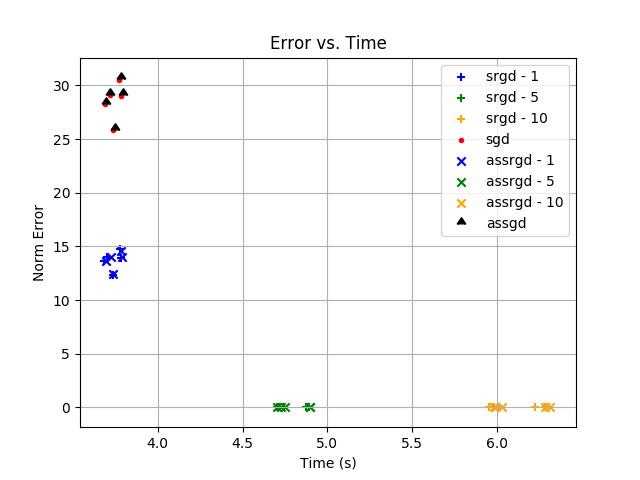
\includegraphics[width=2.5in]{dim-100-batch-500}
    \caption{Comparison of error as a function of compute time for a mini-batch
    of 500 points and a 100 dimensional parameter space.}
    \label{fig:dim10}
\end{figure}
\begin{figure}[!t]
    \centering
    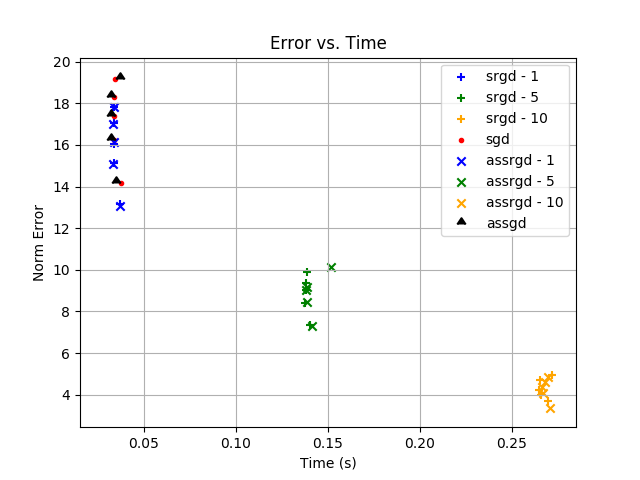
\includegraphics[width=2.5in]{dim-10-batch-500}
    \caption{Comparison of error as a function of compute time for a mini-batch
    of 500 points and a 10 dimensional parameter space.}
    \label{fig:dim10}
\end{figure}
\begin{figure}[!t]
    \centering
    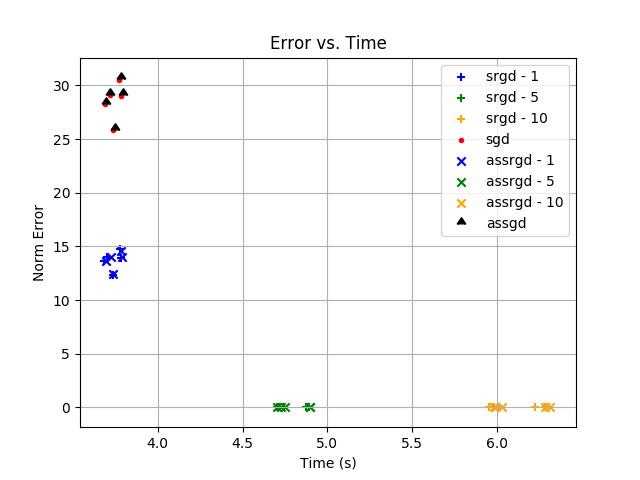
\includegraphics[width=2.5in]{dim-100-batch-1000}
    \caption{Comparison of error as a function of compute time for a mini-batch
    of 1,000 points and a 100 dimensional parameter space.}
    \label{fig:dim10}
\end{figure}
\begin{figure}[!t]
    \centering
    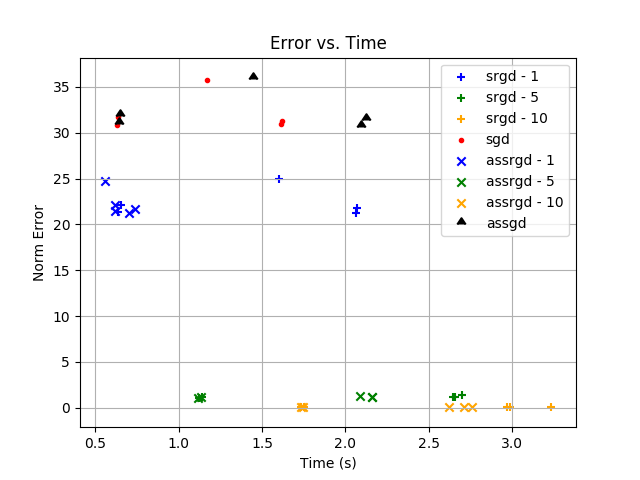
\includegraphics[width=2.5in]{dim-50-batch-500}
    \caption{Comparison of error as a function of compute time for a mini-batch
        of 500 points and a 50 dimensional parameter space.}
    \label{fig:dim50}
\end{figure}

Additionally (Need to add figure/table), it is interesting to note that the
SRGD and ASSRGD methods achieved better accuracy, typically in less time, and
they utilized fewer data points than standard SGD. In other words, they were
able to do more with less information.

% An example of a floating figure using the graphicx package.
% Note that \label must occur AFTER (or within) \caption.
% For figures, \caption should occur after the \includegraphics.
% Note that IEEEtran v1.7 and later has special internal code that
% is designed to preserve the operation of \label within \caption
% even when the captionsoff option is in effect. However, because
% of issues like this, it may be the safest practice to put all your
% \label just after \caption rather than within \caption{}.
%
% Reminder: the "draftcls" or "draftclsnofoot", not "draft", class
% option should be used if it is desired that the figures are to be
% displayed while in draft mode.
%
%\begin{figure}[!t]
%\centering
%\includegraphics[width=2.5in]{myfigure}
% where an .eps filename suffix will be assumed under latex, 
% and a .pdf suffix will be assumed for pdflatex; or what has been declared
% via \DeclareGraphicsExtensions.
%\caption{Simulation results for the network.}
%\label{fig_sim}
%\end{figure}

% Note that the IEEE typically puts floats only at the top, even when this
% results in a large percentage of a column being occupied by floats.


% An example of a double column floating figure using two subfigures.
% (The subfig.sty package must be loaded for this to work.)
% The subfigure \label commands are set within each subfloat command,
% and the \label for the overall figure must come after \caption.
% \hfil is used as a separator to get equal spacing.
% Watch out that the combined width of all the subfigures on a 
% line do not exceed the text width or a line break will occur.
%
%\begin{figure*}[!t]
%\centering
%\subfloat[Case I]{\includegraphics[width=2.5in]{box}%
%\label{fig_first_case}}
%\hfil
%\subfloat[Case II]{\includegraphics[width=2.5in]{box}%
%\label{fig_second_case}}
%\caption{Simulation results for the network.}
%\label{fig_sim}
%\end{figure*}
%
% Note that often IEEE papers with subfigures do not employ subfigure
% captions (using the optional argument to \subfloat[]), but instead will
% reference/describe all of them (a), (b), etc., within the main caption.
% Be aware that for subfig.sty to generate the (a), (b), etc., subfigure
% labels, the optional argument to \subfloat must be present. If a
% subcaption is not desired, just leave its contents blank,
% e.g., \subfloat[].


% An example of a floating table. Note that, for IEEE style tables, the
% \caption command should come BEFORE the table and, given that table
% captions serve much like titles, are usually capitalized except for words
% such as a, an, and, as, at, but, by, for, in, nor, of, on, or, the, to
% and up, which are usually not capitalized unless they are the first or
% last word of the caption. Table text will default to \footnotesize as
% the IEEE normally uses this smaller font for tables.
% The \label must come after \caption as always.
%
%\begin{table}[!t]
%% increase table row spacing, adjust to taste
%\renewcommand{\arraystretch}{1.3}
% if using array.sty, it might be a good idea to tweak the value of
% \extrarowheight as needed to properly center the text within the cells
%\caption{An Example of a Table}
%\label{table_example}
%\centering
%% Some packages, such as MDW tools, offer better commands for making tables
%% than the plain LaTeX2e tabular which is used here.
%\begin{tabular}{|c||c|}
%\hline
%One & Two\\
%\hline
%Three & Four\\
%\hline
%\end{tabular}
%\end{table}


% Note that the IEEE does not put floats in the very first column
% - or typically anywhere on the first page for that matter. Also,
% in-text middle ("here") positioning is typically not used, but it
% is allowed and encouraged for Computer Society conferences (but
% not Computer Society journals). Most IEEE journals/conferences use
% top floats exclusively. 
% Note that, LaTeX2e, unlike IEEE journals/conferences, places
% footnotes above bottom floats. This can be corrected via the
% \fnbelowfloat command of the stfloats package.


\section{Future Work}
A key issue in evaluating the efficacy of this new methodology is determining
whether the algorithm is getting cache hits on the data while training. This is
an extremely low-level process and not as straightforward to measure. Further
compounding the issue is the use of Python makes cache-misses extremely likely
(due to the nature of the Python language). At a high level, almost everything
in Python is an object and so there is a lot of indirection for seemingly simple
Python expressions. This means that by the time we perform an update and go to
recalculate the gradient for the same data point, the data has probably been
evicted from the cache. At this point, it must be refetched from RAM, which is
the exact situation we are trying to avoid with this new approach.\\

The question remains: what can be done? The next step is to move to a
lower-level language such as C or C++ and implement a smaller test problem. Our
intution is that while this started out as a clever approach to squeeze some
additional performance out of various optimization algorithms, it appears to
effectively utilize the L1 or L2 caches the optimization routines will need to
be highly optimized to a point that it is beyond the scope of an average
library user. Take, as a comparison, the BLAS library, which is highly optimized
and makes extensive use of cache-optimized algorithms. The matrix-multiply
routines are substnatially more complicated than the standard approach of three
nested for-loops.\\

The last complicating factor in our approach is that of both hyper-threading and
asynchronous data fetching. In the hyper-threaded setting, the CPU actually
prefetches the data into cache while performing its standard tasks (actually,
these two processes are interleaved) -- this has the effect of removing any
latency from RAM access. That's not to say there is no room for cache
optimization on modern processors, just that it takes quite a bit more planning.
The other related issue is that of asynchronous data fetching. The framework
Caffe [ADD REF] is a great example of this approach. Caffe creates (at least)
two threads, one for main program execution and the other to handle data
fetching. While the model is making its forward and backward passes (training
phase), the data thread is pulling data from the database (which is typically on
disk) into memory, preparing it for use in training. This implementation is
quite efficient, and removes a lot of the latency from data access.

\section{Conclusion}
While we did not achieve the results we were hoping for in this project, a lot
was learned. At a minimum, at this level of optimization having a strong
understanding of the hardware and OS operations is quite important. Making use
of cache optimizations can certainly improve overall runtime, but is much more
complex than we initially thought. It may turn out that these optimzations can
be made, just not at the data load phase of the optimizer.

% conference papers do not normally have an appendix



% use section* for acknowledgment
\ifCLASSOPTIONcompsoc
  % The Computer Society usually uses the plural form
  \section*{Acknowledgments}
\else
  % regular IEEE prefers the singular form
  \section*{Acknowledgment}
\fi




% trigger a \newpage just before the given reference
% number - used to balance the columns on the last page
% adjust value as needed - may need to be readjusted if
% the document is modified later
%\IEEEtriggeratref{8}
% The "triggered" command can be changed if desired:
%\IEEEtriggercmd{\enlargethispage{-5in}}

% references section

% can use a bibliography generated by BibTeX as a .bbl file
% BibTeX documentation can be easily obtained at:
% http://mirror.ctan.org/biblio/bibtex/contrib/doc/
% The IEEEtran BibTeX style support page is at:
% http://www.michaelshell.org/tex/ieeetran/bibtex/
%\bibliographystyle{IEEEtran}
% argument is your BibTeX string definitions and bibliography database(s)
%\bibliography{IEEEabrv,../bib/paper}
%
% <OR> manually copy in the resultant .bbl file
% set second argument of \begin to the number of references
% (used to reserve space for the reference number labels box)
\begin{thebibliography}{1}

\bibitem{bib:xu-assgd}
Y.~Xu, Q.~Lin, T.~Yang, \emph{Accelerated Stochastic Subgradient Methods
under Local Error Bound Condition}, arXiv:1607.01027, 2017

\bibitem{bib:mnist}
Y.~LeCun, C.~Cortes, \emph{MNIST handwritten digit database}, http://yann.lecun.com/exdb/mnist/, 2010

\bibitem{bib:pytorch}
\emph{PyTorch}, https://pytorch.org
\end{thebibliography}




% that's all folks
\end{document}


